\subsection{Ligne de mise à feu}
\label{subsec:ligne_mise_a_feu}

La ligne de mise à feu est conçue pour assurer un allumage fiable et sécurisé du moteur du 2e étage de la fusée. Son objectif est
d'être capable de fournir assez de puissance à l'inflamateur lorsque le séquenceur donne l'odre de la mise à feu.

\begin{figure}[h!]
    \centering
    \begin{subfigure}{\textwidth}
        \centering
        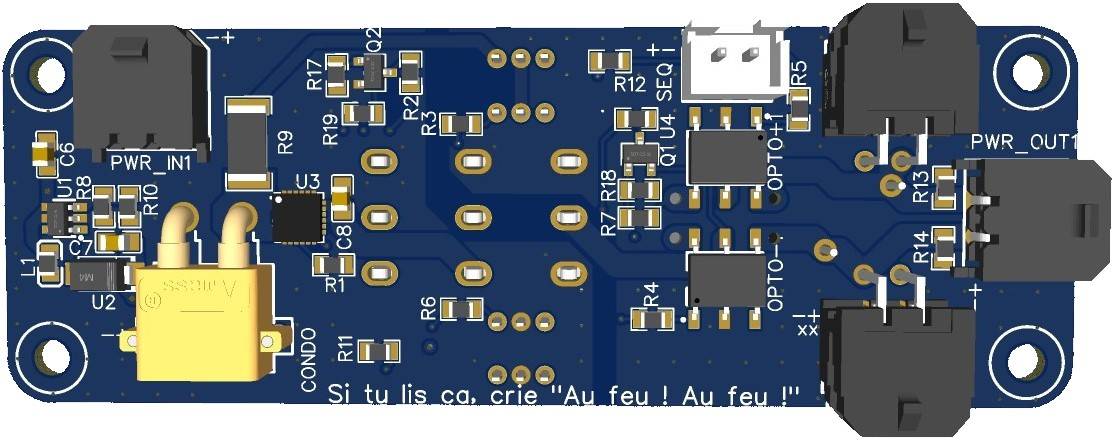
\includegraphics[width=0.6\textwidth]{figures/PCB_Allumage_main.jpg}
        \caption{(côté composants)}
    \end{subfigure}
    \begin{subfigure}{\textwidth}
        \centering
        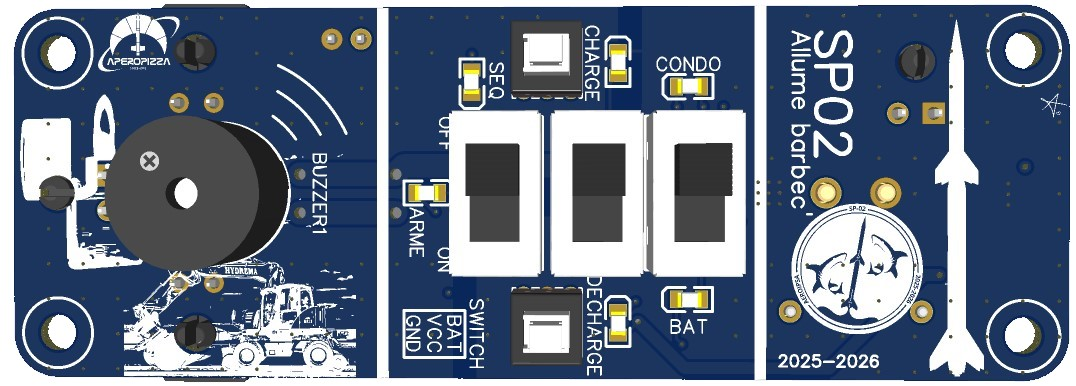
\includegraphics[width=0.6\textwidth]{figures/PCB_Allumage_main_back.jpg}
        \caption{(côté interface)}
    \end{subfigure}
    \caption{Rendu 3D de la carte allumage}
\end{figure}

\newpage
